\documentclass[twoside]{article}
\setlength{\oddsidemargin}{0.25 in}
\setlength{\evensidemargin}{-0.25 in}
\setlength{\topmargin}{-0.6 in}
\setlength{\textwidth}{6.5 in}
\setlength{\textheight}{8.5 in}
\setlength{\headsep}{0.75 in}
\setlength{\parindent}{0 in}
\setlength{\parskip}{0.1 in}
\usepackage{natbib}
\usepackage{amsmath,amsfonts,graphicx}

%
% The following commands set up the lecnum (chap number)
% counter and make various numbering schemes work relative
% to the chap number.
%
\newcounter{lecnum}
\renewcommand{\thepage}{\thelecnum-\arabic{page}}
\renewcommand{\thesection}{\thelecnum.\arabic{section}}
\renewcommand{\theequation}{\thelecnum.\arabic{equation}}
\renewcommand{\thefigure}{\thelecnum.\arabic{figure}}
\renewcommand{\thetable}{\thelecnum.\arabic{table}}

%
% The following macro is used to generate the header.
%
\newcommand{\chap}[5]{
   \pagestyle{myheadings}
   \thispagestyle{plain}
   \newpage
   \setcounter{lecnum}{#1}
   \setcounter{page}{1}
   \noindent
   \begin{center}
   \framebox{
      \vbox{\vspace{2mm}
    \hbox to 6.28in { {\bf SDS 383D: Modeling II
	\hfill Spring 2017} }
       \vspace{4mm}
       \hbox to 6.28in { {\Large \hfill Section #1: #2  \hfill} }
      \vspace{2mm}}
   }
   \end{center}
   \markboth{Section #1: #2}{Section #1: #2}

   
}
%
% Convention for citations is authors' initials followed by the year.
% For example, to cite a paper by Leighton and Maggs you would type
% \cite{LM89}, and to cite a paper by Strassen you would type \cite{S69}.
% (To avoid bibliography problems, for now we redefine the \cite command.)
% Also commands that create a suitable format for the reference list.
%\renewcommand{\cite}[1]{[#1]}
%\def\beginrefs{\begin{list}%
%        {[\arabic{equation}]}{\usecounter{equation}
%         \setlength{\leftmargin}{2.0truecm}\setlength{\labelsep}{0.4truecm}%
%         \setlength{\labelwidth}{1.6truecm}}}
%\def\endrefs{\end{list}}
%\def\bibentry#1{\item[\hbox{[#1]}]}

%Use this command for a figure; it puts a figure in wherever you want it.
%usage: \fig{NUMBER}{SPACE-IN-INCHES}{CAPTION}
\newcommand{\fig}[3]{
			\vspace{#2}
			\begin{center}
			Figure \thelecnum.#1:~#3
			\end{center}
	}
% Use these for theorems, lemmas, proofs, etc.
\newtheorem{theorem}{Theorem}[lecnum]
\newtheorem{lemma}[theorem]{Lemma}
\newtheorem{proposition}[theorem]{Proposition}
\newtheorem{claim}[theorem]{Claim}
\newtheorem{corollary}[theorem]{Corollary}
\newtheorem{definition}[theorem]{Definition}
\newtheorem{exercise}{Exercise}[lecnum]
\newtheorem{example}{Example}[lecnum]
\newenvironment{proof}{{\bf Proof:}}{\hfill\rule{2mm}{2mm}}

% **** IF YOU WANT TO DEFINE ADDITIONAL MACROS FOR YOURSELF, PUT THEM HERE:

\newcommand\E{\mathbb{E}}
\newcommand\Prob{\mathbf{P}}
\newcommand\Q{\mathbf{Q}}
\newcommand\cov{\mbox{cov}}
\begin{document}
\chap{5}{Mixture models}
\maketitle


\section{Mixture models}

So far, we've assumed that our data are conditionally exchangeable given their covariates. In other words, for every unique set of covariates there exists a set of parameters, conditioned on which, the data with those covariates are i.i.d. We used various distributions over functions to learn a distribution over these parameters, for all covariate settings.

A common setting was when our data was normally distributed, with mean $\beta^Tx_i$ and variance $\sigma^2$. If we did not have the covariate values $x_i$, our data would no longer be normally distributed.

\begin{exercise}

  Download the dataset restaurants.csv. This contains profit information for restaurants, based on seating capacity and whether they are open for dinner. Run a Bayesian regression of Profit vs SeatingCapacity and a dummy for DinnerService (you can reuse code from 2.12) (I'd suggest whitening Profit, it will make later prior specification easier). Do the residuals look normal? (e.g.\ plot histograms, qq plots). Now, let's just look at the raw Profit data: Does it look normal?
\end{exercise}

Let's assume we're in the situation where we don't know any of these covariate values. For now, let's ignore the continuous-valued covariate (SeatingCapacity), and try to infer the categorical covariate. Let's say we know that half our restaurants are open for dinner. We could assume that each restaurant is associated with a \textit{latent} indicator variable $Z_i$, that assigns them to one of two groups, so that

$$Z_i \sim \mbox{Bernoulli}(\pi)$$

As in the regression setting, conditioned on the latent variable, we will assume that the observed profits are i.i.d.\ normal. Again, as in the basic regression setting, we will assume the variances of the two normals are the same, but the means are different, i.e.

$$X_i|Z_i=z \sim \mbox{Normal}(\mu_{z}, \sigma^2).$$

If we marginalize over these binary indicators, our observations are assumed to be distributed according to a mixture of two Gaussians:

$$X_i \sim 0.5N(\mu_1,\sigma_1^2) + 0.5(\mu_2,\sigma_2^2)$$

We can then look at the posterior distribution over each indicator variable, conditioned on the class probabilities and parameters:

$$\begin{aligned}\Prob(Z_i = z|X_i, \pi, \mu_1,\sigma^2) \propto& P(Z_i=z|\pi)p(X_i|\mu_z,\sigma^2)\\
  \mbox{so, }\qquad \Prob(Z_i=1|X_i, \pi, \mu_1,\sigma^2) \propto& \pi p(X_i|\mu_1,\sigma^2)\\
  \Prob(Z_i=0|X_i, \pi, \mu_1,\sigma^2) \propto& P(Z_i=0|\pi)p(X_0|\mu_z,\sigma^2)
\end{aligned}$$

Conditioned on the $Z_i$, we can update the means of the Gaussians using conjugacy.

Note that we are not guaranteed to find latent clusters that correspond to the covariate we were expecting! If there is a more parsimonious partitioning of the data, then the posterior will tend to favor that partitioning.

\begin{exercise}
  Let's assume (as is the case if our latent variables correspond to the actual DinnerService covariate) that the class proportions are roughly equal, and fix $\pi=0.5$. Using the conditional distributions $P(Z_i|X_i,\pi,\mu_1,\mu_2,\sigma^2)$ and $p(\mu_k|\{X_i:Z_i=k\}, \theta)$, where $\theta$ are appropriate (shared) prior parameters for $\mu_k$, implement a Gibbs sampler that samples the means and the latent indicator variables. I'd suggest using the parameters of the initial regression to pick your hyperparameters.

  Compare the clustering obtained with the ``true'' clustering due to the DinnerService variable.
\end{exercise}


OK, let's now assume we don't know $\pi$, and that the two classes have different values of $\sigma^2$. Let's put a Beta$(\alpha,\beta)$ prior on $\pi$, since it is conjugate to the Bernoulli distribution. 

\begin{exercise}
  Let's assume we want to integrate out $\pi$. What is the conditional distribution $P(Z_i|Z_{\neg i}, X_i,\mu_1,\mu_2,\sigma_1,\sigma_2,\alpha,\beta)$, where $Z_{\neg i}$ means all the values of $Z$ except $Z_i$?
\end{exercise}

\begin{exercise}
  How about if we want to integrate out all of the continuous variables? What is the conditional distribution $P(Z_i|Z_{\neg i}, X, \theta)$, where $\theta$ is the set of all hyperparameters?
\end{exercise}

\begin{exercise}
  Implement a Gibbs sampler for this new model where we learn the cluster proportions. You can either implement one of the variants in the previous two exercises, or the fully uncollapsed model where we sample $Z$, $\pi$, $\mu_1$, $\mu_2$, $\sigma^2_1$ and $\sigma^2_2$.
\end{exercise}


Let's now consider the case where we have more than two classes. Here, we need to replace our Bernoulli distribution with a multinomial parametrized by some probability vector $\pi$, so that:

$$P(Z_i = k) = \pi_k$$


  Much as the multinomial is the multivariate generalization of the binomial distribution, the Dirichlet($\alpha_1,\dots,\alpha_K$) distribution, which has pdf
  $$\frac{\Gamma(\sum_k \alpha_k)}{\prod_k \Gamma(\alpha_k)} \prod_{k=1}^K \pi_k^{\alpha_k},$$
  is the multivariate generalization of the beta distribution. Here, $\alpha$ is a $D$-dimensional vector where $\alpha_k>0$ and $\sum_k\alpha_k\geq 1$. The expectation of a Dirichlet distribution is given by the normalized parameter vector, $E[\pi] = \frac{(\alpha_1,\dots,\alpha_K)}{\sum_k\alpha_k}$. The absolute magnitude of the parameter acts like an inverse variance: the smaller its values, the further a given sample is from the expected value. Figure~\ref{fig:DirSimp} below shows the pdf of three Dirichlet distributions represented on the 3-simplex, with samples from those distributions
  \begin{figure}
    \begin{center}
      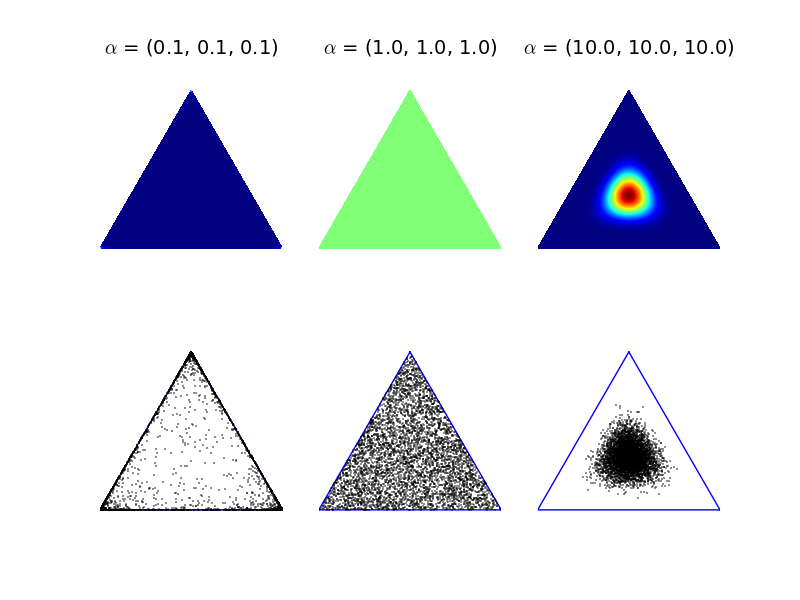
\includegraphics[width=.7\textwidth]{dirichlet-simplex}
      \caption{PDF and samples from three Dirichlet distributions with parameters $\alpha$}
      \label{fig:DirSimp}
    \end{center}
  \end{figure}

\begin{exercise}
 Show that the Dirichlet is conjugate to the multinomial, and derive the posterior predictive distribution

  $$P(Z_{n+1}|Z_{1:n}) = \int_{\mathcal{M}} P(Z_{n+1}|\pi)p(\pi) d\pi$$

  You may find it helpful to note that, if $\pi\sim \mbox{Dirichlet}(\alpha_1,\dots,\alpha_K)$, then $E[\pi] = \frac{(\alpha_1,\dots,\alpha_K)}{\sum_k\alpha_k}$.
\end{exercise}





 \begin{exercise}
   Modify your previous Gibbs sampler to allow multiple classes, and two-dimensional data. Generate some data according to a Dirichlet mixture of 5 Gaussians in $\mathbb{R}^2$, and test your code on it.

\end{exercise}

 \begin{exercise}
   OK, let's try a real dataset! We're going to use a set of images from MNIST. Download the dataset mnist.csv from the data directory, and transform it to be zero mean, unit variance. Each row contains the vectorized pixel values for an image of a digit. The whole dataset contains 100 copies of each digit, with the first 100 being zeros, the next 100 being ones, etc. You can visualize a data point by reshaping it to be 28$\times$28:

   \begin{itemize}
   \item R: \texttt{image(matrix(X[1,],nrow=28))}
   \item Python: \texttt{import matplotlib.pyplot; plt.imshow(X[0,:].reshape(28,28)); plt.show()}
   \item Matlab: \texttt{imshow(reshape(X(1,:),28,28))}
   \end{itemize}

  
   
   The data is 784-dimensional; let's reduce this by running PCA and using the first 50 dimensions.


   Now, try running your Gibbs sampler with 10 classes, and $\alpha_1 =\alpha_2=\dots=\alpha_{10} = 1$. This prior corresponds to a uniform distribution on the 9-simplex. It's fine to use a spherical covariance here... in fact it will work fine if you just have a prior on the means, and fix $\sigma^2=1$.

   Here are some ways you can visualize your output:
   \begin{itemize}
   \item Based on a single sample, plot the recovered clustering vs the ground truth clustering.
   \item Based on a single sample, visualize the mean image for each cluster, by multiplying the mean embedding with the coefficients obtained using PCA.
   \item Over multiple samples, create a co-occurrence matrix with entries being the proportion of the times that the two data points are in the same sample.
   \end{itemize}
 \end{exercise}

 \begin{exercise}[Optional]
   OK, let's try a different likelihood. Let's consider modeling documents. A common modeling assumption is to treat a document as a ``bag-of-words'' -- assuming that all the information is in the words, and none of it is in the ordering. Under this assumption, an appropriate distribution is a multinomial distribution over words, with a Dirichlet prior. Concretely, let:

   $$\begin{aligned}
     \pi \sim& \mbox{Dirichlet}_K(\alpha)\\
     \eta_k \sim& \mbox{Dirichlet}_V(\beta),\qquad k=1,\dots,K\\
     z_i \sim& \mbox{Discrete}(\pi),\qquad i=1,\dots, N\\
     \mathbf{w}_i \sim& \mbox{Multinomial}(\eta_{z_i})
   \end{aligned}$$

   where $N$ is the number of documents, $V$ is the number of words in the dictionary, $K$ is the number of clusters, and $\mathbf{w}_i$ is a $V$-dimensional count vector representing the $i$th document.

   Write out the conditional distributions for a collapsed (i.e.\ integrating out $\pi$ and the $\eta_k$) Gibbs sampler for this model.

 \end{exercise}

 \begin{exercise}[Optional]
   Implement the code. Generate a test set by generating data from a mixture of two multinomials, one with probabilities $(1,1,1,1,9,9,9,9)/40$ and the other with probabilities $(9,9,9,9,1,1,1,1)/40$. Test your code on this dataset, and compare a single sample's clustering pattern with the ground truth values.


   Once you've got it to work on the toy data, try it on some real data! The file \texttt{cora.csv} on Github contains a bag-of-words representation of a collection of 2410 scientific documents from the Cora search engine (taken from the R package \texttt{lda}. Each row corresponds to a document, each column to a word, each element is the number of times that word appears in that document. The list of words is at \texttt{cora\_vocab.csv}. Try clustering them into say 10 clusters. The NIPS dataset on Github contains the text of NIPS papers. Try clustering them into say 10 clusters. Based on a single sample for each cluster, report the 10 most frequently occurring words.
 

 \end{exercise}
\subsection{Admixture models}
 A mixture model for text isn't massively realistic. Consider the NIPS papers: is it really reasonable to separate multiple documents into distinct clusters? It is more likely that two papers share some aspects in common, but differ on others.

 We can use a hierarchical Bayesian formulation to model each document using a mixture model, with a shared prior on the mixing components. Concretely, let
 $$\begin{aligned}
   \theta_i\sim& \mbox{Dirichlet}_K(\alpha),\qquad i=1,\dots,N\\
   \eta_k \sim& \mbox{Dirichlet}_V(\beta),\qquad k=1,\dots,K\\
   z_{i,j} \sim& \mbox{Discrete}(\theta_i),\qquad j=1,\dots, M_i\\
   w_{i,j} \sim& \mbox{Discrete}(\eta_{z_{i,j}}),\end{aligned}$$
 where $M_i$ is the number of words in the $j$th document. This model is commonly known as Latent Dirichlet Allocation \cite{BleNgJor2003}; it is an example of an \textit{admixture} model.
 
 This means that each document is associated with a distribution $\theta_i$ over clusters, and each word is associated with a single cluster.

 \begin{exercise}
   We can construct a collapsed Gibbs sampler for this model by integrating out the $\theta_i$ and the $\eta_k$. Derive the predictive distributions  $p(z_{i,j}|\{z_{\neg i,j}\}, \alpha)$ and $p(w_{i,j}|z_{i,j},z_{\neg i,j},w_{\neg i,j},\beta)$, and hence the conditional distribution $p(z_{i,j}|\mbox{rest})$
 \end{exercise}

 \begin{exercise}
   I'm not going to make you implement this one (although if you want to, feel free!). Instead, let's use the R package \texttt{lda} (sorry Python/R folk! it should be fairly easy to use). The documentation is here: \texttt{https://cran.r-project.org/web/packages/lda/lda.pdf}. Run the Gibbs sampler on the built-in document dataset \texttt{cora}, and report the 5 words with highest probability for each cluster (hint: look at the example under top.topic.words -- note that you might need more iterations than is given in the example, R has a rule that examples have to run quickly, hence the low number in the example). Why is this sort of model commonly called a topic model?
 \end{exercise}
 


 \section{Bayesian nonparametric models}

 When we were modeling the MNIST dataset, we used 10 clusters. This seems reasonable, right -- there are 10 digits! However, if you look at the data, there is a lot of variation within each digit. Maybe we'd be better off using more clusters... but how many?

 One answer to this question is to allow \textit{infinitely} many clusters \textit{a priori}. Each data point can only belong to a single cluster, so there will only be at most $N$ occupied clusters. By allowing infinitely many clusters, we can allow $N$ data points to occupy a random number of clusters. Further, if we see more data, we are not restricted to the previously occupied clusters.

 \begin{exercise}

   To get a feel for this, we can ``approximate'' a model with infinitely many clusters with a model with a large number of clusters. Let's start with a Dirichlet prior on cluster membership, with 100 clusters.

   Sample $\pi\sim \mbox{Dirichlet}_{100}(10,10,\dots,10)$, and then sample 10 cluster indicators $z_i\sim \pi$. Record the list of cluster indicators, e.g.\ $\{1,10,11,11,\dots\}$. Do this 5 times, with a different $\pi$ each time.

   Repeat this with $\alpha = (1,1,\dots,1)$, $\alpha = (0.1,0.1,\dots,0.1)$ and $\alpha=(0.01,0.01,\dots,0.01)$.

   Comment on how the value of $\alpha$ affects your clustering behavior.
 \end{exercise}

   OK, now let's explore some further properties of the Dirichlet distribution. First, we note an important relationship between the Dirichlet distirbution from the gamma distribution: If
   $$\gamma_i \stackrel{\mbox{\small{iid}}}{\sim}\mbox{Gamma}(\alpha_i,\beta)$$
   then
   $$Z = \sum_{i=1}^K \gamma_i \sim \mbox{Gamma}\left(\sum_{i=1}^K\alpha_i,\beta\right)$$
   and
   $$\pi = \left(\frac{\gamma_1}{Z},\dots,\frac{\gamma_K}{Z}\right)\sim \mbox{Dirichlet}(\alpha_1,\alpha_K)$$

   \begin{exercise}
     Using the change-of-variable technique with the transform $(\gamma_1,\dots,\gamma_K)\rightarrow (\pi_1,\dots, \pi_{K-1},Z)$, prove the above result.
   \end{exercise}

   You will probably find this relationship helpful in proving the following
   
   \begin{exercise}[Agglomeration property]
     Show that, if $(\pi_1,\dots, \pi_K) \sim \mbox{Dirichlet}(\alpha_1,\dots,\alpha_K)$, then $(\pi_1+\pi_2,\dots,\pi_K) \sim \mbox{Dirichlet}(\alpha_1+\alpha_2,\alpha_3,\dots,\alpha_K)$.
   \end{exercise}

   %\begin{exercise}[Decimation property]
   %  Let  $(\pi_1,\dots, \pi_K) \sim& \mbox{Dirichlet}(\alpha_1,\dots,\alpha_K)$, and let $\tau \sim \mbox{Beta}(\beta)$. Show that $\tau \pi_1,(1-\tau)\pi_1,\pi_2,\dots,\pi_K) \sim \mbox{Dirichlet}(\beta \alpha_1,(1-\beta)\alpha_1,\alpha_2,\dots, \alpha_K)$. 

   %\end{exercise}


   \begin{exercise}
     Let $\pi\sim \mbox{Dirichlet}_K\left(\frac{\alpha}{K},\dots,\frac{\alpha}{K}\right)$, and assign weight $\pi_k$ to the interval $\left[\frac{k-1}{K},\frac{k}{K}\right)$. Show that, for any partition with breaks at multiples of $\frac{1}{k}$, the distribution over the weights associated with the blocks in the partition will be Dirichlet distributed.
   \end{exercise}

   The Dirichlet process extends this idea to arbitrary partitions. Concretely, the Dirichlet process is a distribution over measures\footnote{If you're not familiar with measure theory, a measure on some space is just a function that assigns a positive number to every subset of that space. So, a probability is a measure. Area is a measure.} on some space $\mathcal{\Omega}$, parametrized by some probability distribution $H$ on $\Omega$ and some positive scalar $\alpha$ such that for any partition $A_1,\dots,A_K$ of $\Omega$, the masses assigned to $A_1,\dots, A_k$ are distributed according to a Dirichlet ($\alpha H(A_1),\dots, \alpha H(A_K)$) distribution. The resulting probability distribution $D$ will have its probability concentrated on infinitely many singletons $D=\sum_{i=1}^\infty \pi_i \delta_{\theta_i}$-- what is known as an atomic probability distribution.

   We can construct a finite dimensional approximation to the Dirichlet process by sampling $\pi\sim\mbox{Dirichlet}_K\left(\frac{\alpha}{K},\dots,\frac{\alpha}{K}\right)$ for some large $\alpha$, and associating each probability $\pi_k$ with a location $\theta_k\sim H$. This distribution will converge weakly to the Dirichlet process as $K\rightarrow \infty$.

   \begin{exercise}
     Return to the MNIST mixture model, and replace your 10-dimensional Dirichlet distribution with a 100-dimensional Dirichlet with parameters $\alpha/100$ for, say, $\alpha=1$. How many clusters does it use (look at a distribution over multiple samples)? Based on a single sample, what do those clusters look like?
   \end{exercise}

   
   
  \bibliographystyle{apalike}
  \bibliography{course}

\end{document}
